%\documentclass{exam}
\documentclass[answers,addpoints]{exam}
\usepackage{amsmath,amssymb,enumerate,float,tikz,etoolbox,ifthen,xcolor,ulem,graphicx, comment,hyperref,multicol,enumerate,makecell,pgfplots,geometry}
\pgfplotsset{compat=1.18}
\usetikzlibrary{decorations.pathreplacing}

\geometry{
  % margin=1in,
  top=0.5in,
  bottom=0.5in,
  left=0.75in,
  right=0.75in,
  letterpaper
}

\definecolor{MyGreen}{rgb}{0.1, 0.4, 0.1}
\definecolor{MyBlue}{rgb}{0.1, 0.1, 0.9}

\AtBeginEnvironment{solution}{\color{MyGreen}}

\newboolean{NoSolutions}

\newcommand\pts[1][2]{\textcolor{MyBlue}{\text{\bf [#1 pts]}}}
\newcommand\pt{\textcolor{MyBlue}{\text{\bf [1 pt]}}}
\newcommand\ds{\displaystyle}

\makeatletter
\renewcommand{\thefigure}{\thequestion.\arabic{figure}}
\@addtoreset{figure}{question}
\makeatother

\setlength\parindent{0in}
\pagestyle{empty}
\begin{document}

\section*{MATH 100 GROUP PROJECT 2: \\Implicit Differentiation and Linear Approximation}

\normalsize

\subsection*{Contributors}

Alexandre \textbf{Boutoille} (22291660) Brennan \textbf{Coetzer} (64702178) Dino \textbf{Lee} (29709300) Andaya \textbf{Vincent} (33234436)

\hrulefill

\subsection*{Reflection Question}

\begin{solution}
  The questions in high school math were more directed towards solving the problem using equations and following the steps whereas the questions in the first group project required a lot more thought and proof both in mathematical equations and graphs as well as written explanations. This required a much deeper understanding of different mathematical concepts rather than just how to apply them.

  Question 2c of Group Project 1 asks us to rank four functions by size, this not only required knowledge of what each function looks like graphically but also how the function behaves over time. Therefore, concepts on how trigonometric functions, exponential functions, and rational functions behave were required to understand the problem and thus solve it.
\end{solution}

\hrulefill

\newpage

\fullwidth{
\subsection*{Assignment questions}}

\begin{questions}
  \question \
  \begin{solution}

    \begin{figure}[H]
      \centering
      \begin{tabular}{@{}l@{}}
        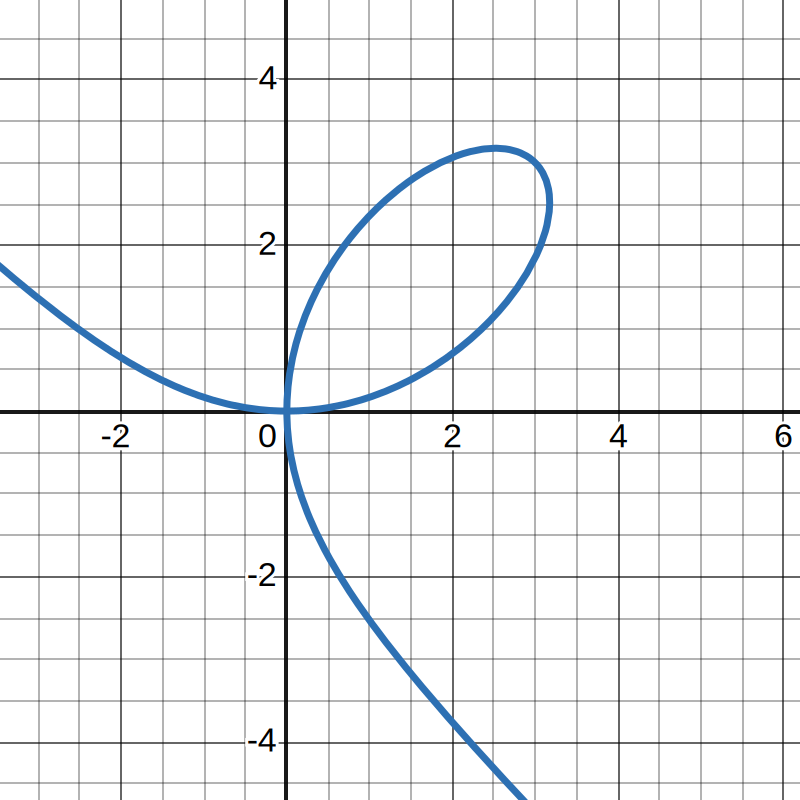
\includegraphics[width=5cm]{desmos-graph.png}
      \end{tabular}
      \caption{$x^3+y^3=6xy$ Graph}
      \label{fig:graph}
    \end{figure}

    \begin{figure}[H]
      \centering
      \begin{tabular}{@{}l@{}}
        $\displaystyle x^3+y^3=6xy$ \\[6pt]
        $\displaystyle (3)^3+(3)^3=6(3)(3)$ \\[6pt]
        $\displaystyle 54=54$ \\[12pt]
        $\displaystyle \frac{d}{dx}3x^2+\frac{dy}{dx}3y^2=\frac{d}{dx}6y+\frac{dy}{dx}6x$ \\[6pt]
        $\displaystyle \frac{dy}{dx}=\frac{2y-x^2}{y^2-2x}$ \\[6pt]
        $\displaystyle \frac{dy}{dx}=\frac{2(3)-(3)^2}{(3)^2-2(3)}$ \\[6pt]
        $\displaystyle =-1$ \\[12pt]
        $\displaystyle L(x)=f(a)+f^\prime(x)(x-a)$ \\[6pt]
        $\displaystyle L(x)=(3)+(-1)(x-3)$ \\[6pt]
        $\displaystyle y=-x+6$ \\
      \end{tabular}
      \caption{1a Mathematical Work}
      \label{fig:1a-math}
    \end{figure}

    It is assumed that $y=f(x)$ if $(3,3)$ exists and has only one tangent line. Although $x=3$ has two values as seen in \ref{fig:graph}, $y=f(x)$ exists locally at $(3,3)$. If $y=f(x)$ could not be written at the point, the tangent line would not exist with a value of $\infty$. This would indicate a graph turning-back on itself Even though the curve fails the VLT, there is only one tangent line in the small region. $\therefore$ the slope is $-1$—a real number—so $y=f(x)$ near $(3,3)$.

    \begin{figure}[H]
      \centering
      \begin{tabular}{@{}l@{}}
        $\displaystyle L(x)=f(a)+f^\prime(a)(x-a)$ \\[6pt]
        $\displaystyle L(1)=3-1(1-3)$ \\[6pt]
        $\displaystyle L(2.5)=3-1(2.5-3)$ \\[6pt]
        $\displaystyle =3.5$ \\
      \end{tabular}
      \caption{1b Mathematical Work}
      \label{fig:1b-math}
    \end{figure}

    The single-step estimate for $b$ is inaccurate as linear approximations are accurate the more you deviate from where the approximation was derived from. Linear approximations find points on a tangent line, hence the further you deviate the more accuracy decreases. Regardless, since the curve is concave downwards as seen in \ref{fig:graph}, the real value at $x=2.5$ will be less than the overestimate provided by the approximation.

  \end{solution}

  % -------------------------------------------------------

  \question \
  \begin{solution}

    \begin{figure}[H]
      \centering
      \begin{tabular}{r r r r r r}
        \hline
        \multicolumn{1}{c}{$n$} &
        \multicolumn{1}{c}{$x_n$} &
        \multicolumn{1}{c}{$y_n$} &
        \multicolumn{1}{c}{$m_n$} &
        \multicolumn{1}{c}{$x_{n+1}$} &
        \multicolumn{1}{c}{$y_{n+1}$} \\
        \hline
        0 & 3.0000 & 3.0000 & -1.0000 & 2.9000 & 3.1000 \\
        1 & 2.9000 & 3.1000 & -0.5801 & 2.8000 & 3.1580 \\
        2 & 2.8000 & 3.1580 & -0.3485 & 2.7000 & 3.1929 \\
        3 & 2.7000 & 3.1929 & -0.1886 & 2.6000 & 3.2117 \\
        4 & 2.6000 & 3.2117 & -0.0658 & 2.5000 & 3.2183 \\
        5 & 2.5000 & 3.2183 & 0.0348 & 2.4000 & 3.2148 \\
        \hline
      \end{tabular}
      \caption{2a Calculations Table}
      \label{fig:2a-vi-table}
    \end{figure}

    \begin{figure}[H]
      \centering
      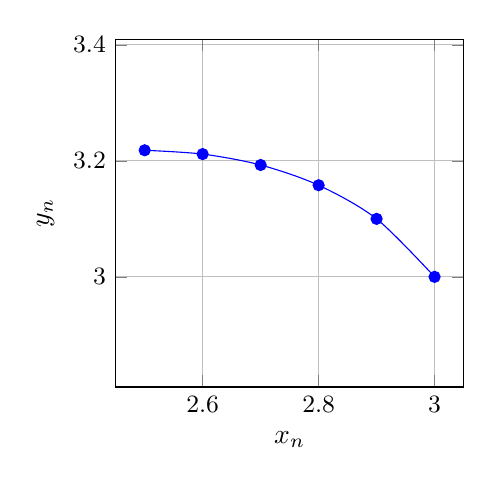
\begin{tikzpicture}
        \begin{axis}[
            axis equal,
            xlabel=$x_n$,
            ylabel=$y_n$,
            grid=both,
            width=6cm,
            height=6cm,
            xmin=2.45, xmax=3.05,
            ymin=3.0, ymax=3.22,
            tick label style={font=\small}
          ]

          \addplot[blue, mark=*,thin,smooth] coordinates {
            (3.0000, 3.0000)
            (2.9000, 3.1000)
            (2.8000, 3.1580)
            (2.7000, 3.1929)
            (2.6000, 3.2117)
            (2.5000, 3.2183)
          };
        \end{axis}
      \end{tikzpicture}
      \caption{2a $x_n$ vs $x_y$ plot}
      \label{fig:2a-vii-plot}
    \end{figure}

    The approximate value for b produced in this process is $b \approx 3.218927$, this is slighter closer to the actual value than the value of $3.5$ obtained in Question 1. The accuracy improved because a new tangent line is used every time we move closer to $2.5$ from $3$. However, as we are approximating the value of $y_n+1$ using mn, the tangent line still slightly overshoots the actual value of $y_n+1$ of the curve for every step, resulting in error. These errors then accumulate, resulting in an approximate value of $b$ that is higher than the actual value.

    \begin{figure}[H]
      \centering
      \begin{tabular}{r r r r r r}
        \hline
        \multicolumn{1}{c}{$n$} &
        \multicolumn{1}{c}{$x_n$} &
        \multicolumn{1}{c}{$y_n$} &
        \multicolumn{1}{c}{$m_n$} &
        \multicolumn{1}{c}{$x_{n+1}$} &
        \multicolumn{1}{c}{$y_{n+1}$} \\
        \hline
        0 & 3.0000 & 3.0000 & -1.0000 & 2.9500 & 3.0500 \\
        1 & 2.9500 & 3.0500 & -0.7649 & 2.9000 & 3.0882 \\
        2 & 2.9000 & 3.0882 & -0.5976 & 2.8500 & 3.1181 \\
        3 & 2.8500 & 3.1181 & -0.4689 & 2.8000 & 3.1416 \\
        4 & 2.8000 & 3.1416 & -0.3646 & 2.7500 & 3.1598 \\
        5 & 2.7500 & 3.1598 & -0.2772 & 2.7000 & 3.1737 \\
        6 & 2.7000 & 3.1737 & -0.2018 & 2.6500 & 3.1837 \\
        7 & 2.6500 & 3.1837 & -0.1354 & 2.6000 & 3.1905 \\
        8 & 2.6000 & 3.1905 & -0.0761 & 2.5500 & 3.1943 \\
        9 & 2.5500 & 3.1943 & -0.0223 & 2.5000 & 3.1954 \\
        10 & 2.5000 & 3.1954 & 0.0270 & 2.4500 & 3.1941 \\
        \hline
      \end{tabular}
      \caption{2b Calculations Table}
      \label{fig:2b-table}
    \end{figure}

    \begin{figure}[H]
      \centering
      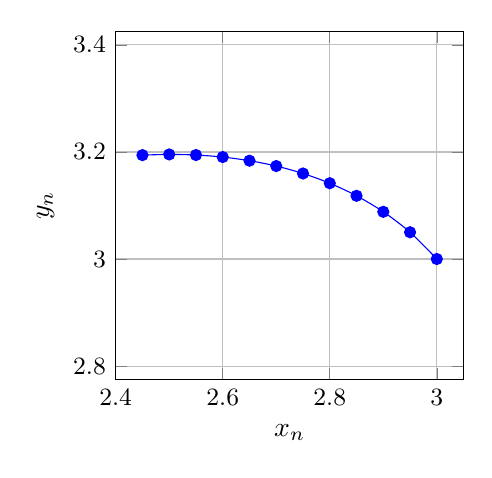
\begin{tikzpicture}
        \begin{axis}[
            axis equal,
            xlabel=$x_n$,
            ylabel=$y_n$,
            grid=both,
            width=6cm,
            height=6cm,
            xmin=2.40, xmax=3.05,
            ymin=3.0, ymax=3.20,
            tick label style={font=\small}
          ]

          \addplot[blue, mark=*,thin,smooth] coordinates {
            (3.0000, 3.0000)
            (2.9500, 3.0500)
            (2.9000, 3.0882)
            (2.8500, 3.1181)
            (2.8000, 3.1416)
            (2.7500, 3.1598)
            (2.7000, 3.1737)
            (2.6500, 3.1837)
            (2.6000, 3.1905)
            (2.5500, 3.1943)
            (2.5000, 3.1954)
            (2.4500, 3.1941)
          };
        \end{axis}
      \end{tikzpicture}
      \caption{2b $x_n$ vs $x_y$ plot}
      \label{fig:2b-plot}
    \end{figure}

    Changing $h$ from $0.1$ to $0.05$ caused the approximate value of $b$ to go from $b \approx 3.218927$ to $b \approx 3.195442$. This is even closer to the actual value of $b \approx 3.174607$, meaning that using a smaller $h$ improved the accuracy of the approximation.

    This is because we must calculate a new $y_n$ more frequently when using a smaller $h$, thus each tangent line calculated is closer to the curve and the error produced on each step becomes smaller. This results in a smaller error overall and thus a closer approximation to the actual value of $b$.

  \end{solution}

  %\hrulefill
  % -------------------------------------------------------
  \question \
  \begin{solution}

    \begin{figure}[H]
      \centering
      \begin{tabular}{@{}l@{}}
        $\displaystyle \frac{dy}{dx}=\frac{2(0)-(0^2)}{(0)^2-2(0)}$ \\[6pt]
        $\displaystyle =0=\text{DNE}$ \\[6pt]
      \end{tabular}
      \caption{3a Mathematical Work}
      \label{fig:3a-math}
    \end{figure}

    At $(0,0)$, multiple paths pass-through. It's a point of self-intersection, so has no (WORD). $\therefore$ we can't reliably use the tangent line method.

    The derivative found in \ref{fig:1a-math} can't really be simplified at $(0,0)$ using L'Hôpital's rule as seen in \ref{fig:3a-math}. $\therefore$ you cannot get a slope for the tangent line, so the iterative tangent line method at $(0,0)$ can't be used.

    A linear approximation cannot be used to find $(p,q)$ when $q=1$ at $(0,0)$. This is because the slope of the tangent line is an indeterminate form, as there is an intersection of paths at $(0,0)$ on the graph. We cannot use iterative tangent line techniques to estimate anything if we start at $(0,0)$, as the initial slope is an indeterminate form.

    Since no singular tangent line exists at $(0,0)$ when the graph intersects, as there are multiple paths leading to $(0,0)$, issues will arise when solving for the slope.

    There are essentially multiple tangent lines at $(0,0)$ since multiple path lead there. This means there are multiple coordinates that the linear approximation could give at this point for $(a,b)$ when $a=1$, and $(p,q)$ with $q=1$. Generally, you cannot apply this approaching starting at $(0,0)$.

    \begin{figure}[H]
      \centering
      \begin{tabular}{@{}l@{}}
        $\displaystyle \frac{0}{0}$ \\[6pt]
      \end{tabular}
      \caption{3d Mathematical Work}
      \label{fig:3d-math}
    \end{figure}

    We recognize the intermediate form tells use we cannot start at the point $(0,0)$, so instead, we start at a point that is incredibly close to $(0,0)$, but not quite there. We can use the estimated point $(0.05,0)$. We don't know what the true corresponding y value with $x=0.05$ is, but we know it is so close to $0$ that we can essentially assume that it is zero for the purpose of our approximation, since it is just an approximation. Then, using (x0,y0)=(0.05,0), we can start the iterative tangent line approach, increasing in small steps of $h=0.05$ for accuracy to give us coordinates of points using tangent lines incredibly close to $(0,0)$, but not quite at $(0,0)$. The math demonstrated shows the steps to solve for the slope of one tangent line near $(0,0)$, but not quite at $(0,0)$. This will give us a very good approximation of values, overcoming issues we identify with starting at $(0,0)$. The points intersect perfectly at $(0,0)$, but not at points incredibly close to $(0,0)$, so we can still use the iterative method at those points. If we wanted to find an estimate of the for an $0$ value of $1$, we would continue this iterative process until we get to an $x$-value of $1$. This is how we would essentially solve these types of problems while overcoming the issue of starting at $(0,0)$. To make this mathematical approach more accurate, we could make h increment in smaller steps like $0.01$ instead of $0.05$. The most accurate increment would be incrementing by values infinitely close to $0$, all the way to the desired value, as there would be an infinite amount of tangent line approximations, giving an essentially perfectly accurate value for whatever point we try to approximate. Unfortunately, this approach would also take an infinite amount of time to calculate, making it ineffective to say the least. The core concept to consider is that having smaller increments of $h$ will produce smaller changes in the $x$ and $y$ values, making the approximations stay closer to the curve between each iteration of the process. This gives the most accurate final value, but takes more steps.

  \end{solution}

  % -------------------------------------------------------

  \hrulefill
  % -------------------------------------------------------

  % -------------------------------------------------------

\end{questions}
\end{document}

%-------------------------------------------------------------
%-------------------------------------------------------------
%-------------------------------------------------------------
